\documentclass[10pt,tikz,border=1mm]{standalone} 
\usepackage{mathpazo}
\usepackage[T1]{fontenc}
\usetikzlibrary{positioning,calc,arrows.meta}
\tikzstyle{arrow}=[-{Stealth[scale=1.25]},thin,text=black,font=\normalsize,draw=black]
\tikzstyle{process}=[rectangle,minimum height=1.5cm,minimum width=2cm,fill=black!5,draw=black,very thick]
\tikzstyle{empty}=[circle,inner sep=0pt,fill=none]
\tikzstyle{hdist}=[node distance=2.5cm]
\tikzstyle{number}=[circle,fill=black!10,font=\footnotesize,inner sep=0.5mm,draw=black,thin]
\begin{document}
	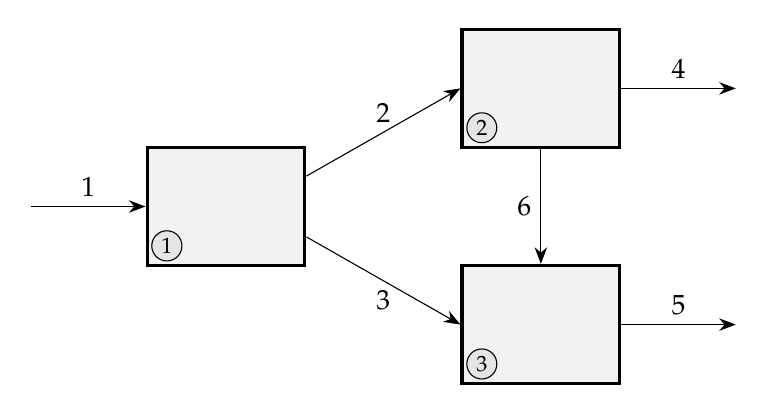
\begin{tikzpicture}
		%\draw[step=1cm,black!20,very thin] (-1,-2) grid (7,2);
		\node [empty] (V0)  {};
		\node [process] (N1) [right of=V0,hdist]{};
		\node [process,at={(6.5,1.5)}] (N2) {};
		\node [process,at={(6.5,-1.5)}] (N3) {};
		\node [empty] (W1) [right of=N2,hdist] {};
		\node [empty] (W2) [right of=N3,hdist] {};
		\draw [arrow] (V0) -- node[above]{1} (N1);
		\coordinate (N1a) at ($(N1.east)!0.5!(N1.north east)$);
		\coordinate (N1b) at ($(N1.east)!0.5!(N1.south east)$);
		\draw [arrow] (N1a) -- node[above]{2} (N2.west);
		\draw [arrow] (N1b) -- node[below]{3} (N3.west);
		\draw [arrow] (N2) -- node[above]{4} (W1);
		\draw [arrow] (N3) -- node[above]{5} (W2);
		\draw [arrow] (N2) -- node[left]{6} (N3);
		\node[number,at={(1.75,-0.5)}] {1};
		\node[number,at={(5.75,1)}] {2};
		\node[number,at={(5.75,-2)}] {3};
	\end{tikzpicture}
\end{document}		
	